\chapter{Konzeption}
% TODO: weiter schreiben
Dieses Kapitel beschreibt alle notwendigen Schritte für die Konzeption der angewandten Methode, außerdem werden die Datensätze
und die verwendeten Tools präsentiert.

\section{Image Colorization als Multimodales Problem}
Konventionelle automatische Methoden zielen darauf ab, die Farben für ein generiertes Bild so nah wie möglich an das originale Bild vorherzusagen.
Diese Methoden verwenden ein MSE Loss, das Vorhersagen, die weit von den originalen Farbwerten entfernt liegen, stärker bestraft, als Farbwerte
die dichter an den originalen Farbwerten liegen. Das führt, wie bei \ref{subsection:verwandte-arbeiten} beschrieben zu entsättigten Bildern.
Die Gründe für diese Ergebnisse lassen sich dadurch erklären dass verschiedene Objekte verschiedene Farben besitzen können.

Wenn die multimodalität des Problems berücksichtigt wird, werden Ergebnisse die nicht dem Original entsprechen, ebenfalls als valide Bilder
enkannt. Das wird erreicht indem jedes Pixel klassifiziert wird, anstatt die Distanz zwischen dem Original und dem vorhergesagten zu berechnen.

Die gewählte Methode dieser Arbeit berücksichtigt die multimodalität von Image Colorization und behandelt das Problem als Klassifikation.

\section{Farbraum}
Der Standard Farbraum der Bilder für die Methode dieser Arbeit ist der RGB\footnote{Rot, Grün, Blau}-Farbraum.
Der RGB-Farbraum hat einige Nachteile, die es kompliziert
machen mit diesem Farbraum zu arbeiten. Einer der Nachteile ist, dass das Graustufenbild sich schwer von den Farbkanälen trennen lässt. Ein anderer
Nachteil ist, dass die Farbinformationen in drei Farbkanäle kodiert sind, was die Komplexität eines Modells erhöht. Aus diesem Grund
werden die Bilder für das Preprocessing und die Methode in den Lab-Farbraum konvertiert. Für die Darstellung der Ergebnisse werden die Bilder
von dem Lab-Farbraum in den RGB-Farbraum umgewandelt.
\\
\\
Im Lab-Farbraum können die Farbkanäle ``ab'' problemlos vom Belichtungskanal ``L'' getrennt werden. Der Belichtungskanal ``L''
enthält das Graustufenbild, das in den CNN eingespeist wird.

\begin{figure}[H]
  \vspace{1cm}
  \centering
  \begin{subfigure}
    \centering
    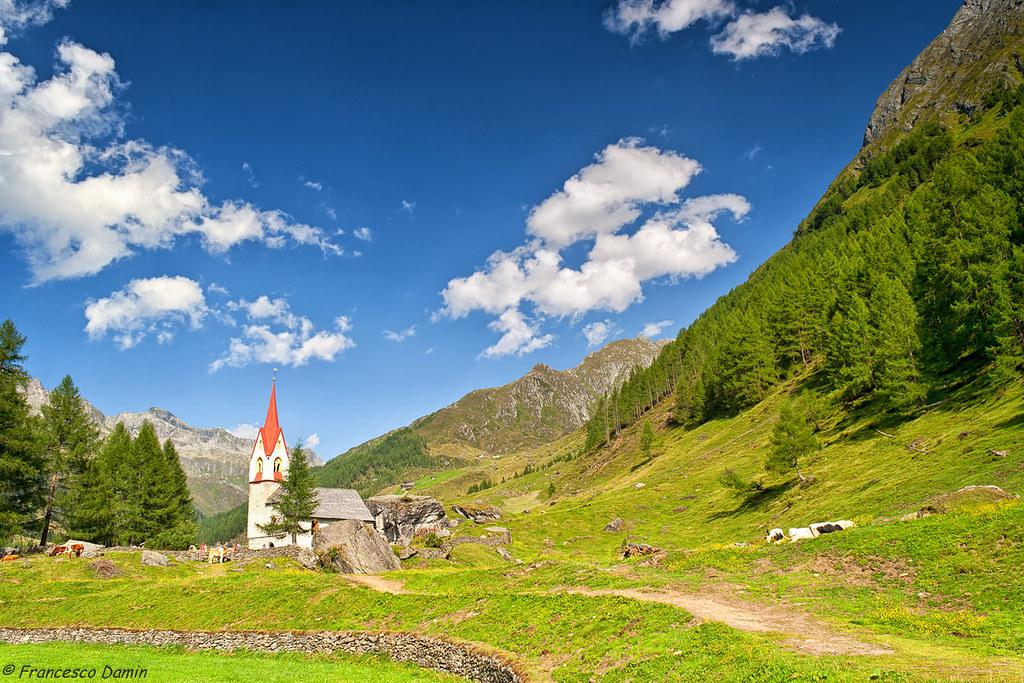
\includegraphics[width=.35\textwidth]{resources/colorspace/image.jpg}
  \end{subfigure}
  \begin{subfigure}
    \centering
    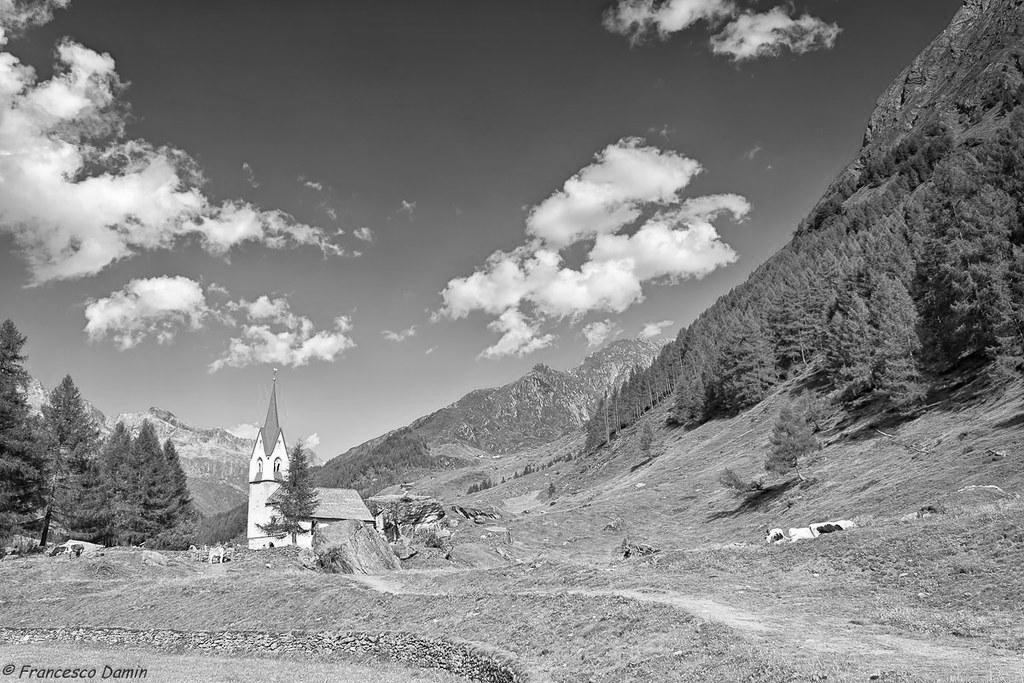
\includegraphics[width=.35\textwidth]{resources/colorspace/grayscale.png}
  \end{subfigure}


  \begin{subfigure}
    \centering
    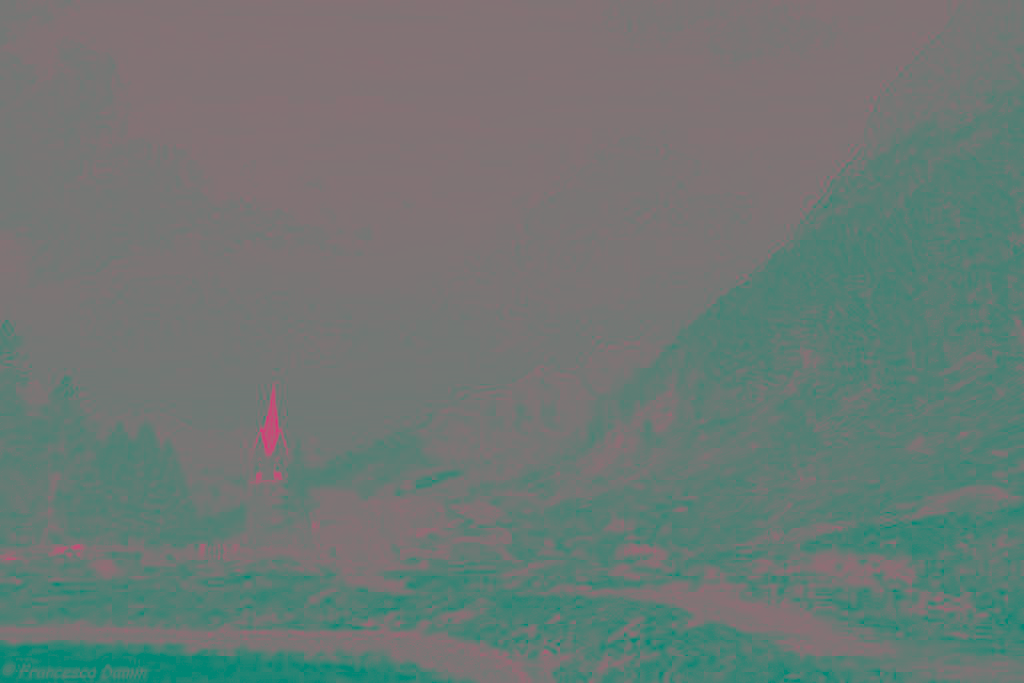
\includegraphics[width=.35\textwidth]{resources/colorspace/a_channel.png}
  \end{subfigure}
  \begin{subfigure}
    \centering
    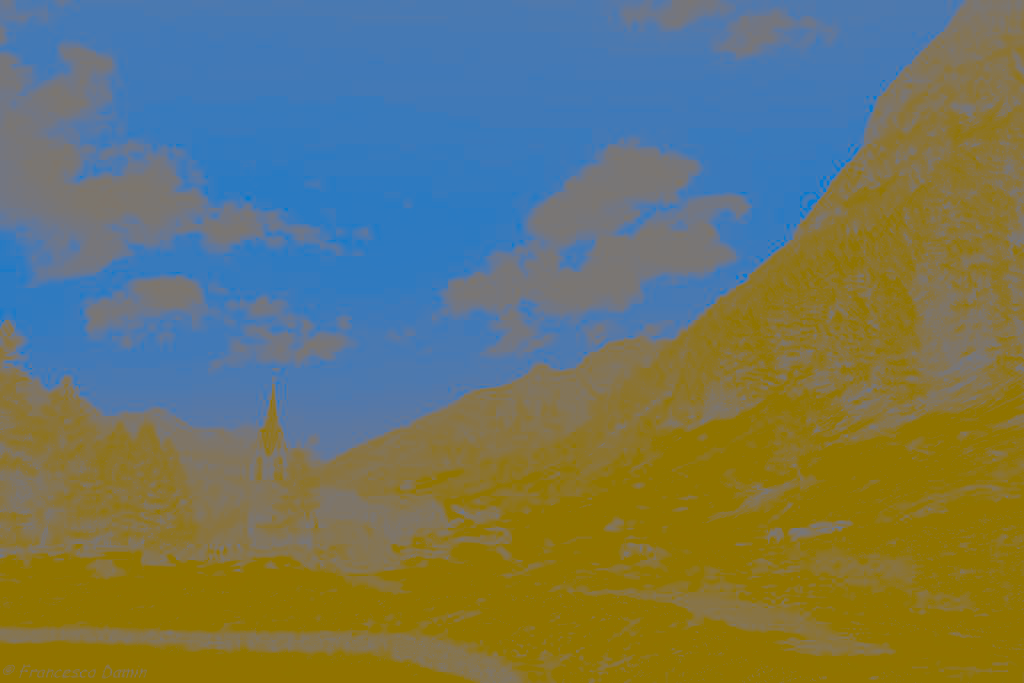
\includegraphics[width=.35\textwidth]{resources/colorspace/b_channel.png}
  \end{subfigure}
  \caption{Original Bild in RGB oben links, Belichtungskanal ``L'' oben rechts, Farbkanal ``a'' unten links und Farbkanal ``b'' unten rechts.}
  \label{image:farbraum}
\end{figure}


\section{Binning}\label{section:binning}
Binning ist eine Technik, die für die Bildverarbeitung verwendet wird. Binning wird, im Kontext von Image Colorization, als Eingruppierung
von naheliegenden Farben definiert. Die Farben werden in gleich große Intervalle aufgeteilt. Diese Intervalle bezeichnet man im englischen als
``\gls{bin}s''. Jedes dieser Intervalle wird durch einen \gls{bin} Index repräsentiert, somit reduziert sich die Anzahl der Klassen die vorhergesagt werden
können.

Als Beispiel für die Veranschaulichung wird der normalisierte Lab-Farbraum in 36 gleich große \gls{bin}s unterteilt. Da die Farbinformationen
in den ``ab'' Farbkanälen kodiert sind, werden nur diese 2 Farbkanäle in \gls{bin}s klassifiziert. Auf der Abbildung \ref{image:bins} ist der Farbkanal
``a'' auf der x-Achse und der Farbkanal ``b'' auf der y-Achse abgebildet. Die Quadrate repräsentieren die \gls{bin}s. Die obere Zahl in den Bins
symbolisiert die $xy$ Koordinaten auf dem \gls{grid}, die untere, unterstrichene Zahl symbolisiert den Bin Index.
Die $xy$ Koordinaten sind Bedeutsam für die Berechnung der Bins.

\begin{figure}[H]
  \centering
  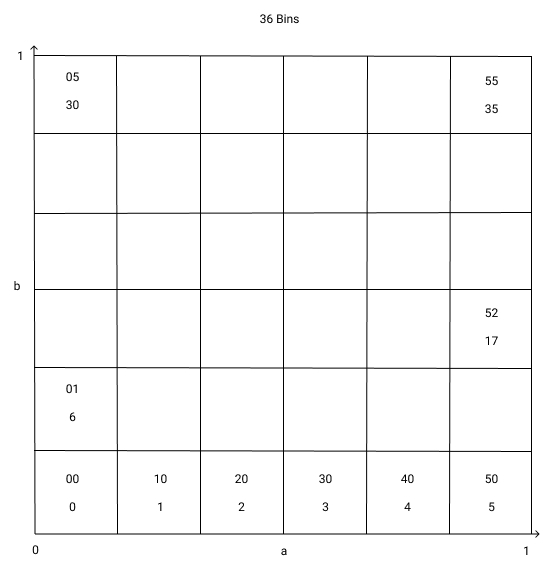
\includegraphics[width=0.7\textwidth]{resources/bins/bins.jpg}
  \caption{
    \gls{grid} mit 36 bins. Die x-Achse bildet die Werte des Farbkanals ``a'' und die y-Achse die Werte des Farbkanals ``b'' ab. (Eigene Darstellung)
  }
  \label{image:bins}
\end{figure}

Für die Methoden dieser Arbeit wurden nur symmetrische \gls{grid}s verwendet, so ergibt zum Beispiel ein $6 \times 6$ Grid 36 Bins und
ein $18 \times 18$ Grid 324 Bins.

Die Umwandlung von Bin zu Farbe muss für die Ergebnisse des Netzwerks ebenfalls vorgegeben sein. Für dieses Problem werden vor dem
Training die Farben von jedem Pixel aus den Trainingsbildern in Bins klassifiziert. Jeder Bin wird durch eine Liste mit je zwei Listen,
für den jeweiligen Farbkanal, repräsentiert. Jeder Pixelwert wird zur entsprechenden Bin Liste hinzugefügt. Anschließend wird der Modus
und der Durchschnitt jedes Farbkanals, der unter jedem Bin klassifizierten Farben, ausgerechnet. Am Ende beinhaltet jeder Bin eine Liste mit je zwei
Werten, auf dem Nulltem Index der Wert für den Farbkanal ``a'' und auf dem ersten Index der Wert für den Farbkanal ``b''. Es werden zwei separate
Dateien erzeugt, eins für den Modus und eins für den Durchschnitt.
\\
\\
Für die Umwandlung von Bin zu Farbe werden die jeweiligen Werte für jeden Farbkanal eines Bins von der jeweiligen Datei abgeguckt. Es kann zwischen
dem Durchschnitt und dem Modus ausgewählt werden. Der Durchschnitt verhält sich ähnlich wie ein Modell trainiert mit dem MSE Loss und der Modus
würde Ergebnisse mit einem rötlichen Farbton liefern. Als Lösung für dieses Problem schlägt Zhang et al. den ``annealed mean'' vor \cite{zhang2016colorful}.
Der ``annealed mean'' versucht einen Kompromiss zwischen dem Durchschnitt und dem Modus zu finden. Dieser Kompromiss wird durch einen
Temperatur Parameter ($T$) reguliert. In der vorliegenden Arbeit wird eine von den ``annealed mean'' inspirierten Methoden implementiert.
Die Methode wird wie folgt implementiert:

\begin{equation}
  \begin{gathered}
    D = K_{mode} - K_{mean} \\
    \hat{y}_{K} = K_{mode} - (D * T)
  \end{gathered}
\end{equation}

wobei $K$ ein Farbkanal ist, $D$ die Distanz zwischen Durchschnitt und Modus, $T$ ein Temperaturwert zwischen 0 und 1 und $\hat{y}_{k}$ die
endgültige Farbe für den Farbkanal $K$ ist.
Ein Temperaturwert von 1 würde den Durchschnitt ergeben, wohingegen ein Temperaturwert von 0, den Modus nicht verändert.

\section{Netzwerkarchitektur}
Die Netzwerkarchitektur ist ein wichtiger Faktor der u.a. die Ergebnisse beeinflusst. Um die Methoden zu vergleichen ist es wichtig ein
leichtes Convolutional Neural Network, das wenige Parameter besitzt, schnell zu trainieren ist und gute Ergebnisse liefert, zu verwenden.
\\
\\
Das Ziel von dem Netzwerk ist es, ein Graustufenbild als Input zu bekommen und eine Wahrscheinlichkeitsverteilung für alle Bins per Pixel vorherzusagen.
Das Output Volumen hat die Dimensionen $ W_{Input} \times H_{Input} \times n\_bins $, wobei $W$ und $H$ die Breite und Höhe des Bildes sind und
$n\_bins$ eine Wahrscheinlichkeitsverteilung für alle Bins pro Pixel ist. Dieser Ansatz wird auch bei Image Segmentation Problemen genutzt, wobei ein Bild
in das Netzwerk eingespeist wird und eine Segmentation map, mit eine Klasse per Pixel, als Output erzeugt wird. In der Regel wird jeder Klasse eine
bestimmte Farbe zugeordnet, was die Objekte klassifiziert und trennt. In dem Fall von Image Colorization bekommt jedes Pixel in dem Output Volumen
eine Wahrscheinlichkeitsverteilung für alle Bins, die in eine Farbe umgewandelt wird.
\\
\\
Die Methoden von Zhang et al. \cite{zhang2016colorful} verwenden ein \gls{CNN}, das ein Graustufenbild als Input entgegennimmt und ein Volumen mit
einer Wahrscheinlichkeitsverteilung für alle Bins per Pixel generiert. Diese Netzwerkarchitektur besteht aus Blöcken mit jeweils 2 oder 3 Convolutional
und ReLU Layers, gefolgt von einer Batch Normalization Layer. Batch Normalization ist eine Regularisierungstechnik, die die Werte in einer Hidden Layer
normalisiert, bevor sie in die nächste Layer weitergereicht werden. Das Netzwerk hat keine Pooling Layers, alle Änderungen in der Auflösung werden durch
Downsampling oder Upsampling zwischen Blöcken erreicht.
\\
Diese Netzwerkarchitektur ist sehr herausfordernd für die GPU\footnote{Graphics Processing Unit}, was die Batch Größe und Trainingszeit stark beeinflusst.
\\
\\
Aus diesem Grund orientiert sich die Netzwerkarchitektur dieser Arbeit an der Netzwerkarchitektur von Billaut et al. \cite{billaut2018colorunet}.
Sie verwenden eine angepasste Version von einem U-net Convolutional Neural Network \cite{ronneberger2015unet}.

\subsection{U-net}\label{section:u-net}
Ein U-net ist ein Autoencoder mit Skip Connections und Transposed Convolutions als Upsampling Methode das bei Image Segmentation angewendet wird.
Im Vergleich zu konventionellen Autoencoder können der Encoder und Decoder nicht getrennt voneinander verwendet werden. Die Skip Connections
ermöglichen fein-granuläre Details in dem Output Volumen wiederherzustellen und helfen mit dem Vanishing Gradient Problem während Backpropagation.
Skip Connections konkatenieren bestimmte Layers aus dem Encoder mit Layers aus dem Decoder, mit den gleichen Dimensionen.
\\
\subsection{Aufbau eines U-nets}\label{section:aufbau-u-net}
Ein U-net besteht, wie ein Autoencoder, aus einem Encoder und Decoder Teil. Der Encoder besteht aus sogenannten ``ConvBlocks''. ConvBlocks
bestehen aus 2 Convolutional Layers gefolgt von Batch Normalization und ReLU. Den ConvBlocks folgt
eine Pooling Layer, die die Dimensionen des Volumens verringert. Der Decoder besteht aus ConvBlocks gefolgt von Transposed Convolutions,
die die Dimensionen von dem Volumen wieder vergrößern. Die letzte Layer ist ein $1 \times 1$ Convolutional Layer, die das Output Volumen generiert.
Skip Connections konkatenieren ConvBlocks aus dem Encoder mit Transposed Convolutions aus dem Decoder mit der gleichen Dimensionen.

\begin{figure}[H]
  \centering
  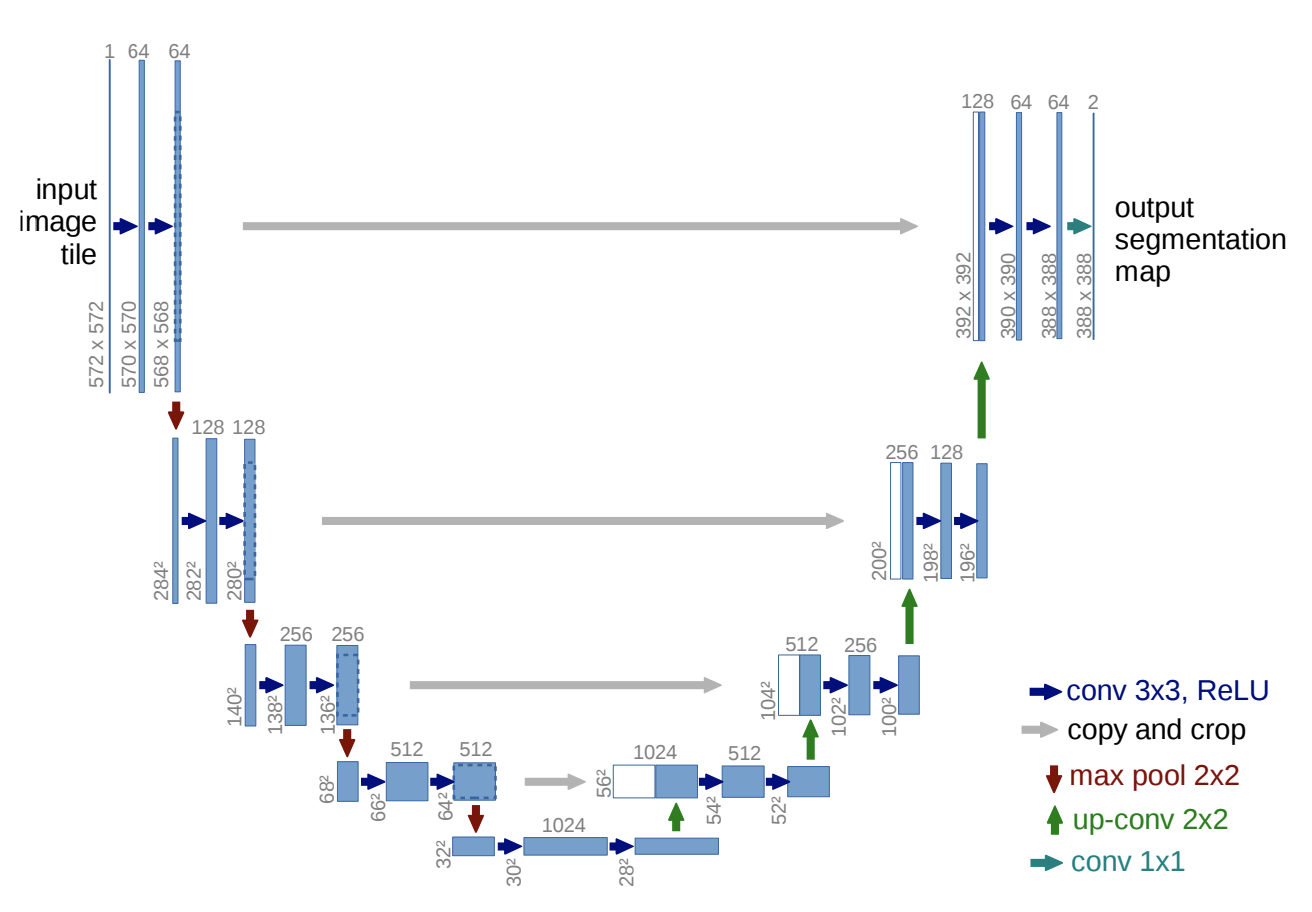
\includegraphics[width=0.85\textwidth]{resources/networks/unet.png}
  \caption{
    U-net Architektur (Beispiel für $32 \times 32$ Pixel in der niedrigsten Auflösung). Jede blaue Box entspricht einer multi-Kanal Feature Map.
    Die Tiefe der Feature Maps ist gekennzeichnet durch die Zahl über der Box. Die Breite und Höhe ist durch die Zahl unten links erkennbar.
    Die weißen Boxen repräsentieren die kopierten Feature Maps. Die Pfeile bestimmen die verschiedenen Operationen.
    \cite{ronneberger2015unet}
  }
  \label{image:unet}
\end{figure}

\section{Datensätze}
Um das Netzwerk zu trainieren werden bedeutsame Bilder mit der gleichen Thematik gebraucht.
Ein Vorteil von Image Colorization ist, dass jedes Bild für das trainieren
verwendet werden kann, da nur die Graustufen Version davon gebraucht wird.

Um die Methode zu prüfen werden 3 Datensätze benutzt, die verschiedene Auflösungen und Themen beinhalten.

Als erstes wird ein Spiel–Datensatz von $ 32 \times 32 $ Bildern generiert. Dieser setzt sich aus 3 geometrischen Objekten und 3 Farben pro
Objekt zusammen. Die geometrischen Objekte sind ein Rechteck, ein Kreis und ein Dreieck pro Bild, die in jeweils eine der 3 Farben eingefärbt sind.
Die Bilder haben einen einheitlichen schwarzen Hintergrund. Der Datensatz kann unter folgendem Link\footnote{\url{https://drive.google.com/file/d/197egEFSMLVq4cspScwdhp1sIk51YWT1U/view?usp=sharing}} gefunden werden.

\begin{figure}[H]
  \centering
  \vspace{1cm}
  \begin{subfigure}
    \centering
    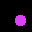
\includegraphics[width=.15\textwidth]{resources/dataset/dummy/circle21.png}
  \end{subfigure}
  \begin{subfigure}
    \centering
    
\includegraphics[width=.15\textwidth]{resources/dataset/dummy/circle68.png}
  \end{subfigure}
  \begin{subfigure}
    \centering
    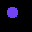
\includegraphics[width=.15\textwidth]{resources/dataset/dummy/circle71.png}
  \end{subfigure}

  \begin{subfigure}
    \centering
    
\includegraphics[width=.15\textwidth]{resources/dataset/dummy/rectangle32.png}
  \end{subfigure}
  \begin{subfigure}
    \centering
    
\includegraphics[width=.15\textwidth]{resources/dataset/dummy/rectangle46.png}
  \end{subfigure}
  \begin{subfigure}
    \centering
    
\includegraphics[width=.15\textwidth]{resources/dataset/dummy/rectangle66.png}
  \end{subfigure}

  \begin{subfigure}
    \centering
    
\includegraphics[width=.15\textwidth]{resources/dataset/dummy/triangle41.png}
  \end{subfigure}
  \begin{subfigure}
    \centering
    
\includegraphics[width=.15\textwidth]{resources/dataset/dummy/triangle49.png}
  \end{subfigure}
  \begin{subfigure}
    \centering
    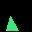
\includegraphics[width=.15\textwidth]{resources/dataset/dummy/triangle51.png}
  \end{subfigure}
  \caption{Beispiel von Trainingsbildern mit einer der möglichen Farben pro Klasse}
  \label{image:dummy}
\end{figure}

Der Datensatz besteht aus 2664 Bildern für das Training und 324 Bildern für die Validierung.
Dieser Datensatz dient als Beweis für das funktionieren der Methode und hilft bei der Entwicklung und Optimierung des Netzwerks.
\\
\\
Als zweites werden 12 Klassen des CIFAR-100\footnote{CIFAR-100: https://www.cs.toronto.edu/~kriz/cifar.html} Datensatzes verwendet. CIFAR-100 ist
ein öffentlich verfügbarer Datensatz, der von Krizhevsky et al. erstellt wurde. Der Datensatz setzt sich aus 100 Klassen mit jeweils 600
Bildern pro Klasse zusammen, außerdem sind die 100 Klassen in 20 Superklassen gruppiert. Der Datensatz wird in 50000 Bildern für das Training und
10000 Bildern für die Validierung aufgeteilt. Einige Beispiele für Klassen sind \textit{apples}, \textit{palm} oder \textit{bee}.
Die Bilder haben ebenfalls einer Auflösung von $ 32 \times 32 $.

Da es äußerst aufwändig wäre ein Modell, dass jedes Objekt aus dem CIFAR-100 Datensatz richtig erkennt und einfärbt,
von Null auf zu trainieren, werden
nur bestimmte Klassen für das Training verwendet. Diese Klassen sind: \textit{apples}, \textit{sunflower}, \textit{rose}, \textit{cloud},
\textit{maple\_tree}, \textit{oak\_tree}, \textit{pine\_tree}, \textit{willow\_tree}, \textit{palm\_tree},
\textit{mountain}, \textit{forest} und \textit{sea}.
Alle Klassen haben Gemeinsamkeiten, was das erlernen von Merkmalen erleichtert im Gegensatz zu einem sehr allgemeinen Datensatz.
\\
\\
Abschließend wird ein komplexerer und hochauflösender Datensatz verwendet, der Naturbezogene Bilder enthält. Ziel ist es, ein Netzwerk zu
trainieren, dass Bilder aus der Natur einfärben kann. Dieses besteht aus 3 Datensätzen von
Kaggle\footnote{Kaggle: \url{https://www.kaggle.com/}} und GitHub\footnote{Github: \url{https://github.com/}}.
Der erste ist der ``Landscape Pictures''\footnote{\url{https://www.kaggle.com/arnaud58/landscape-pictures}} Datensatz von Arnaud Rougetet, von diesem
Datensatz werden alle Bilder verwendet. Der zweite Datensatz ist
``Landscape Classification''\footnote{\url{https://www.kaggle.com/huseynguliyev/landscape-classification}} von Huseyb Guliyev, hiervon werden nur
die Klassen \textit{forest}, \textit{glacier}, \textit{mountain} und \textit{sea} verwendet. Der letzte Datensatz ist der ``Landscapes dataset''
\footnote{\url{https://github.com/ml5js/ml5-data-and-models/tree/master/datasets/images/landscapes}} von ml5js auf GitHub. Von diesem Datensatz wurden
die Klassen \textit{field}, \textit{forest}, \textit{lake}, \textit{mountain} und \textit{road} verwendet. Des Weiteren werden alle Bilder entfernt,
die keine öffentliche Lizenz haben.
\\
Der komplette Datensatz besteht aus 8 Klassen und hat insgesamt
12479 Bilder, 10120 für das Training und 2359 für das Testen. Die 8 Klassen sind: \textit{field}, \textit{forest}, \textit{glacier},
\textit{lake}, \textit{mountain}, \textit{road}, \textit{sea} und ``ohne Kategorie''.
Die Klasse ``ohne Kategorie'' beinhaltet die Bilder aus dem ``Landscape Pictures'' Datensatz. Die Klassen sind für das Training und
die Methode nicht relevant, da jedes Pixel in Bins klassifiziert wird. Der finale Datensatz wird für den Rest der
Arbeit ``Landscape Datensatz'' genannt und kann unter folgendem Link\footnote{\url{https://drive.google.com/file/d/1o73BaE-CYnmtEQgwN427znk1yizrwEsy/view?usp=sharing}} gefunden werden.

\section{Image Preprocessing und Augmentation}
Für das optimale Training und die besten Ergebnisse werden die Bilder vorverarbeitet. Außerdem werden Techniken von Image Augmentation angewendet.
Der Spiel–Datensatz und die 12 Klassen von CIFAR-100 werden für das Training mit einer Wahrscheinlichkeit von 50\% horizontal gespiegelt.
\\
Da der Landscape Datensatz Bilder mit verschiedenen Auflösungen beinhaltet, werden alle Bilder auf $ 128 \times 128 $ angepasst. Das
reduziert die Trainingszeit und die Komplexität des Datensatzes.
Für das Training werden pro Bild 4 zusätzliche augmentierte Bilder generiert. Zunächst werden die Bilder zufälligerweise um $\pm 30$ Grad rotiert,
anschließend wird die Größe der Bilder auf einen Wert zwischen 0 und 30\% geändert.
Nachdem dieser Schritt abgeschlossen ist, werden die Bilder horizontal gespiegelt und abschließend nochmal Vertikal gespiegelt.
Nach der Image Augmentation besteht der Trainings Datensatz aus 50600 Bildern.

\section{Tools}
Um die Methode zu realisieren werden einige Tools genutzt. Für die Implementierung wird das Framework
PyTorch\footnote{https://pytorch.org/}\label{tool:pytorch} verwendet. PyTorch ist ein Open-Source Framework basierend auf Python für Machine Learning und
Deep Learning. Es wurde vom Facebook AI Research Team entwickelt und erschien im Jahr 2016. Zum Zeitpunkt der Verfassung dieser Arbeit ist
die Version 1.6.0 die aktuellste. Für die Farbraum Konvertierung wird die ``scikit-image'' Bibliothek eingesetzt und für die Image Augmentation
wurde die Bibliothek ``imgaug'' ausgewählt. Des Weiteren werden Hilfsbibliotheken wie ``numpy'' und ``matplotlib'' angewendet.
\\
\\
Das Trainieren von den Modellen wird, aufgrund des hohen Rechenaufwands, auf zwei verschiedenen Plattformen durchgeführt. Die Modelle mit den
$32 \times 32$ Bildern werden auf Google Colab\footnote{https://colab.research.google.com/} trainiert. Google Colab ist eine Plattform von
Google, die es ermöglicht Experimente im Browser mit einer Hochleistungsgrafikkarte (Nvidia Tesla P100) kostenlos umzusetzen. Für das Modell mit den
$128 \times 128$ Bildern
wird das Curious Containers (CC) Framework\footnote{https://www.curious-containers.cc/} benutzt. Curious Containers ermöglicht eine
gleichzeitige Durchführung von verschiedenen Experimenten in einem Cluster von Hochleistungsrechnern.


